\documentclass[]{article}
\usepackage{lmodern}
\usepackage{amssymb,amsmath}
\usepackage{ifxetex,ifluatex}
\usepackage{fixltx2e} % provides \textsubscript
\ifnum 0\ifxetex 1\fi\ifluatex 1\fi=0 % if pdftex
  \usepackage[T1]{fontenc}
  \usepackage[utf8]{inputenc}
\else % if luatex or xelatex
  \ifxetex
    \usepackage{mathspec}
  \else
    \usepackage{fontspec}
  \fi
  \defaultfontfeatures{Ligatures=TeX,Scale=MatchLowercase}
\fi
% use upquote if available, for straight quotes in verbatim environments
\IfFileExists{upquote.sty}{\usepackage{upquote}}{}
% use microtype if available
\IfFileExists{microtype.sty}{%
\usepackage[]{microtype}
\UseMicrotypeSet[protrusion]{basicmath} % disable protrusion for tt fonts
}{}
\PassOptionsToPackage{hyphens}{url} % url is loaded by hyperref
\usepackage[unicode=true]{hyperref}
\hypersetup{
            pdfborder={0 0 0},
            breaklinks=true}
\urlstyle{same}  % don't use monospace font for urls
\usepackage{graphicx,grffile}
\makeatletter
\def\maxwidth{\ifdim\Gin@nat@width>\linewidth\linewidth\else\Gin@nat@width\fi}
\def\maxheight{\ifdim\Gin@nat@height>\textheight\textheight\else\Gin@nat@height\fi}
\makeatother
% Scale images if necessary, so that they will not overflow the page
% margins by default, and it is still possible to overwrite the defaults
% using explicit options in \includegraphics[width, height, ...]{}
\setkeys{Gin}{width=\maxwidth,height=\maxheight,keepaspectratio}
\IfFileExists{parskip.sty}{%
\usepackage{parskip}
}{% else
\setlength{\parindent}{0pt}
\setlength{\parskip}{6pt plus 2pt minus 1pt}
}
\setlength{\emergencystretch}{3em}  % prevent overfull lines
\providecommand{\tightlist}{%
  \setlength{\itemsep}{0pt}\setlength{\parskip}{0pt}}
\setcounter{secnumdepth}{0}
% Redefines (sub)paragraphs to behave more like sections
\ifx\paragraph\undefined\else
\let\oldparagraph\paragraph
\renewcommand{\paragraph}[1]{\oldparagraph{#1}\mbox{}}
\fi
\ifx\subparagraph\undefined\else
\let\oldsubparagraph\subparagraph
\renewcommand{\subparagraph}[1]{\oldsubparagraph{#1}\mbox{}}
\fi

% set default figure placement to htbp
\makeatletter
\def\fps@figure{htbp}
\makeatother


\date{}

\begin{document}

\section{Chap.6 Color Image Processing}\label{header-n0}

\textbf{Fullcolor}: acquired with a fullcolor sensor\\
 \textbf{Pseudocolor}: assigned colors to a particular monochrome
intensity or range of intensities.

\(\quad\quad\)Some of the gray-scale methods are directly applicable to
color images.

\subsection{6.1 Color Fundamentals}\label{header-n7}

Intensity for achromatic light\\
 gray level for black-to-grays-to-white.

\emph{Radiance} from the source, \emph{luminance} by the observer,
subjective \emph{brightness}

\(\quad\quad\)It is important to keep in mind that having three specific
primary color wavelengths fro the purpose of standardization deos not
mean that these three fixed RGB components acting alone can generate all
spectrum colors.

Primary colors of light: RGB\\
 Primary colors of pigments/colorants: magenta, cyan, yellow

\(\quad\quad\)CRT: array of triangular dot patterns of
electron-sensitive phosphor that produce different colors. In the case
of LCD, light filters are used to produce the three primary colors of
light.

\(\quad\quad\)Color characteristics: \emph{brightness}, \emph{hue} (an
attribute associated with the dominant wavelength in a mixture of light
waves, like yellow, red, orange), \emph{saturation} (the relative purity
or the amount of white light mixed with a hue).

\emph{Chromaticity}: \emph{Hue}, \emph{saturation}\\

\href{https://en.wikipedia.org/wiki/CIE_1931_color_space\#Tristimulus_values}{\emph{Tristimulus}}
\href{https://en.wikipedia.org/wiki/CIE_1931_color_space\#CIE_xy_chromaticity_diagram_and_the_CIE_xyY_color_space}{CIE
chromaticity diagram} \emph{color gamut}: a range of colors produced by
RGB monitors

\subsection{6.2 Color Models}\label{header-n27}

\(\quad\quad\)A \emph{color model (color space, color system)} is a
specification of a coordinate system and a subspace within that system
where each color is represented by a single point.

The RGB Color Model

\begin{figure}
\centering
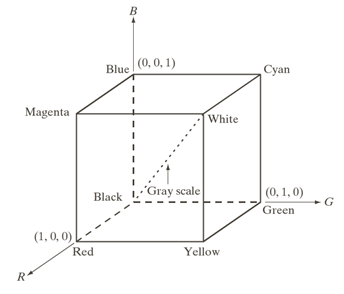
\includegraphics{D:/Documents/GitHub/Commentarii/Digital Image Process Gonzales/1524381382329.png}
\caption{}
\end{figure}

\emph{pixel depth}: the number of bits used to represent eahc pixel in
RGB space.

216 colors out of the 256 colors are de facto standard for \emph{safe
colors}. The safe-color cube has only valid colors on the surface cube.

The CMY and CMYK Color Models

\(\quad\quad\)Most devices that deposit colored pigments on paper such
as color printers and copiers, require CMY data input or perform an RGB
to CMY conversion.

\[\pmatrix{C\\M\\ Y}=\pmatrix{1\\1\\1}-\pmatrix{R\\G\\B}\]

A fourth color, black, combined with C M Y is added.

The HSI Color Model

Practical for human interpretation.

\emph{Hue}: the angle by which a point rotates around the black-white
axis, from red, through yellow, green, cyan, blue, magenta and back to
red. Undefined for a saturation of zero (white, black, and pure grays).
\emph{Brightness} (Intensity): the axis\\
 \emph{Saturation}: distance from the axis

\subsection{6.3 Pseudocolor Image Processing}\label{header-n50}

\(\quad\quad\)For human visualization and interpretation. Humans can
discern thousands of color shades and intensities, compared to only two
dozen or so shades of gray.

Intensity Slicing

Gray scale \([0,L-1]\), \(P\) planes perpendicular to the intensity axis
and \(0<P<L-1\), partitioning the gray scale into \(P+1\) intervals,
\(V_1, V_2,...,V_{P+1}\).

\[f(x,y)=c_k \quad \text{if}\ f(x,y)\in V_k\]

Intensity to Color Transformations

\begin{figure}
\centering
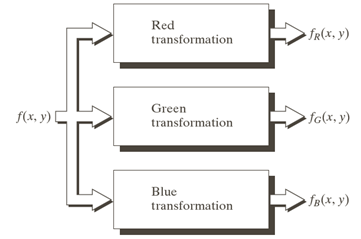
\includegraphics{D:/Documents/GitHub/Commentarii/Digital Image Process Gonzales/1524385570429.png}
\caption{}
\end{figure}

E.g. \(f_R(x,y)\), \(f_G(x,y)\) , \(f_B(x,y)\) are sinusoids of
different phases.

\begin{figure}
\centering
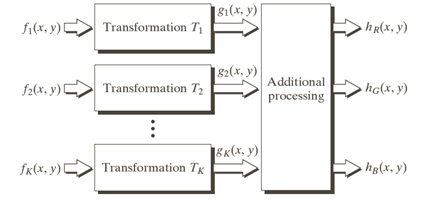
\includegraphics{D:/Documents/GitHub/Commentarii/Digital Image Process Gonzales/1524386227249.png}
\caption{}
\end{figure}

Sometimes it is of interest to combine several monochrome images into a
single color composite.

\subsection{6.4 Basics of Full-Color Image Processing}\label{header-n66}

\(\quad\quad\)The results of individual color component processing are
not always equivalent to direct processing in color vector space.

\subsection{6.5 Color Transformations}\label{header-n69}

\[g(x,y)=T[f(x,y)]\]

where the pixel values here are \emph{triplets} or \emph{quartets}.

\[s_i=T_i(r_1,r_2,...,r_n)\]

where \(r_i\) and \(s_i\) are variables denoting the color compoents of
\(f(x,y)\) and \(g(x,y)\) at any point \((x,y)\), \(n\) is the nubmer of
color components and \(\{T_1, T_2,..., T_n\}\) is a set of
\emph{transformation} or \emph{color mapping functions} that operate on
\(r_i\) to produce \(s_i\).

Color Complements

\(\quad\quad\)The hues directly opposite one another on the \emph{color
circile} are called \emph{complements}.

\begin{figure}
\centering
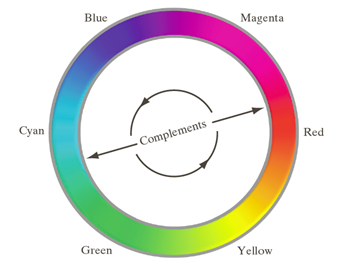
\includegraphics{D:/Documents/GitHub/Commentarii/Digital Image Process Gonzales/1524474472347.png}
\caption{}
\end{figure}

Color complements are useful for enhancing detail that is embedded in
dark regions of a color image, particularly when the regions are
dominant in size.

\begin{figure}
\centering
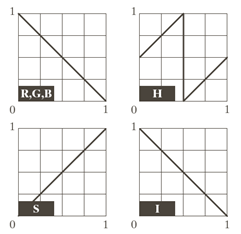
\includegraphics{D:/Documents/GitHub/Commentarii/Digital Image Process Gonzales/1524474884362.png}
\caption{}
\end{figure}

The RGB complement transformation here do not have a straightforward HSI
space equivalent.

Color Slicing

\(\quad\quad\)Highlighting a specific range of colors in an image.

Approaches: \\

\begin{enumerate}
\def\labelenumi{\arabic{enumi}.}
\item
  display the colors of interest so that they stand out from the
  background 
\item
  use the region defined by the colors as a mask for further processing
\end{enumerate}

\(\quad\quad\)One of the simplest way to slice a color image is to map
the colors outside some range of interest to a nonprominent neutral
color.

\[s_i=\begin{cases}0.5 &\text{if } Dist(r,a)>D_0\\
r_i&\text{otherwise}\end{cases}\]

where \(Dist(r,a)\) is a distance measure and \(a\) is a prototypical
color.

Tone and Color Corrections

\href{https://en.wikipedia.org/wiki/Tints_and_shades}{Tints, Shades and
Tones}\\
 \href{https://color-wheel-artist.com/hue/}{Hue, Tint, Tone and Shade}
\href{https://en.wikipedia.org/wiki/Color_balance}{Color Balance}\\

Most common use in photo enhancement and color reproduction.

\textbf{CIELAB}

\(\quad\quad\) The \emph{L*a*b color space} is colorimetric (colors
perceived as matching are encoded identically, perceptually uniform
(color differences among various hues are perceived uniformly) and
device indipendent.

\emph{Tonal range, key-type, high-key, low-key, middle-key}

\textbf{Tonal transformations}: The idea is to adjust the image's
brightness and contrast to provide maximum detail over a suitable range
of intensities. In the RGB and CMYK sapces this means mapping all three
or four color components with the same transformation function; in the
HSI color space, only the \emph{intensity} component is modified.

\textbf{Color balancing}: determined objectively by analyzing with a
color spectrometer a known color in an image, accurate visual
assessments are possible when white areas where the RGB components are
present. Skin tones also are excellent subjects for visual color
assessments.

Histogram Processing

\(\quad\quad\)The gray-level histogram processing transformations can be
applied to color images in an automated way. It is reasonably successful
at handling low-, high-, and middle-key images. It is generally unwise
to histogram equalize the components of a color image independently,
which results in erroneous color. The HSI color space is ideally suited
to this type of approach, which can be performed by equalizing only the
intensity component.

\(\quad\quad\)The intensity equalization process do not alter the values
of hue and saturation of the image, it does impact the overall color
perception.

\section{Chap. 9 Morphological Image Processing}\label{header-n126}

\(\quad\quad\)\emph{Mathematical morphology}: a tool for extracting
image components that are useful in the representation and description
of region shape. Tools such as morphology and related concepts are a
cornerstone of the mathematical foundation that is utilized for
extracting meaning from an image.

\subsection{9.1 Preliminaries}\label{header-n129}

The \emph{reflection} of a set \(B\):
\(\hat{B}=\{w|w=-b\ for\ b\in B\}\)

The \emph{translation} of a set \(B\) by point \(z=(z_1,z_2)\), denoted
by \((B)_z\): \((B)_z=\{c|c=b+z,\ \text{for}\ b\in B\}\)

\emph{structuring elements (SEs)}: small sets or subimages used to probe
an image under the study for properties of interest. An operation is on
a set is defined using a structuring element.

\subsection{9.2 Erosion and Dilation}\label{header-n136}

Erosion

With \(A\) and \(B\) as sets in \(Z^2\) , the \emph{erosion} of \(A\) by
\(B\), defined as

\[A\ominus B=\{z|(B)_z\subseteq A\}\]

or

\[A\ominus B=\{z|(B)_z\cap A^c=\varnothing \}\]

Set \(B\) is assumed to be a structuring element. We can view
\emph{erosion} as a morphological filtering operation in which image
details smaller than the structuring element are filtered.

\begin{figure}
\centering
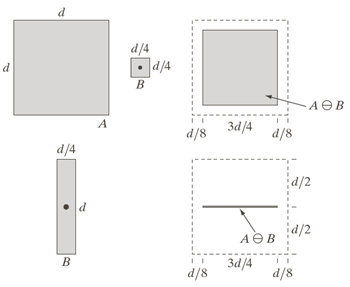
\includegraphics{D:/Documents/GitHub/Commentarii/Digital Image Process Gonzales/1524414290676.png}
\caption{}
\end{figure}

Dilation

With \(A\) and \(B\) as sets in \(Z^2\) , the \emph{dilation} of \(A\)
by \(B\), defined as

\[A\oplus B=\{z|(\hat{B})_z\cap A\neq\varnothing\}\]

or

\[A\oplus B=\{z|(\hat{B})_z\cap A\subseteq A \}\]

\begin{figure}
\centering
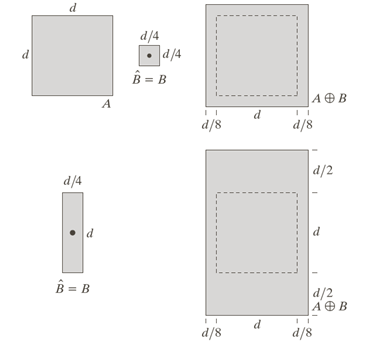
\includegraphics{D:/Documents/GitHub/Commentarii/Digital Image Process Gonzales/1524414299919.png}
\caption{}
\end{figure}

\(\quad\quad\)One of the simplest applications of dilation is for
bridging gaps. One immediate advantage of the morphological approach
over the lowpass filter method is that the morphological method resulted
directly in a binary image.

Duality

\(\quad\quad\)Erosion and dilation are duals of each other w.r.t. set
complementation and reflection.

\[(A\ominus B)^c=A^c\oplus \hat{B}\\
(A\oplus B)^c=A^c\ominus \hat{B}\]

Assume \(\hat{B}=B\), we can obtain the erosion of an image by \(B\)
simply by dilating its background with the same structuring element and
complementing the result.

\subsection{9.3 Opening and Closing}\label{header-n165}

\(\quad\quad\) \emph{Opening} generally smoothes the contour of an
object, breaks down isthmuses and eliminates thin protrusions.
\emph{Closing} generally fuses narrow breaks and long thin gulfs,
eliminates small holes and fills gaps in the contour.

\(\quad\quad\)The \emph{opening} of set \(A\) by structuring element
\emph{B}, defined as

\[A\circ B=(A\ominus B)\oplus B=\bigcup\{(B)_z|(B)_z\subseteq A\}\]

Erosion of \(A\) by \(B\), followed by a dilation of the result by \(B\)

\begin{figure}
\centering
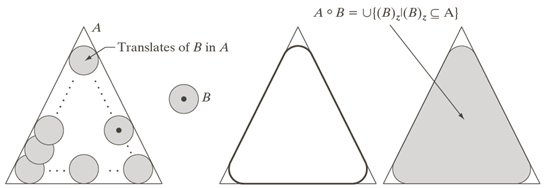
\includegraphics{D:/Documents/GitHub/Commentarii/Digital Image Process Gonzales/1524495249963.png}
\caption{}
\end{figure}

\(\quad\quad\)The \emph{closing} of set \(A\) by structuring element
\(B\), defined as

\[A\ \yen\ B=(A\oplus B)\ominus B\]

\begin{figure}
\centering
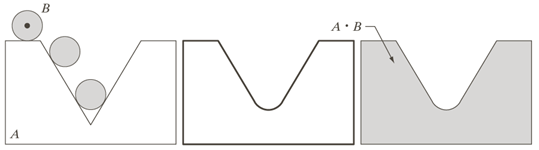
\includegraphics{D:/Documents/GitHub/Commentarii/Digital Image Process Gonzales/1524495465168.png}
\caption{}
\end{figure}

\begin{figure}
\centering
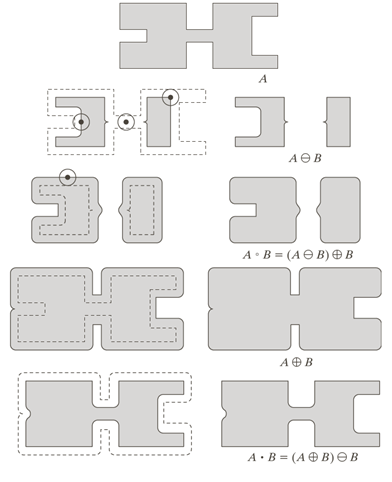
\includegraphics{D:/Documents/GitHub/Commentarii/Digital Image Process Gonzales/1524495725371.png}
\caption{}
\end{figure}

\textbf{Duality}

\[(A\ \yen B)^c=(A^c\circ\hat{B})\\
(A\circ B)^c=(A^c\ \yen\ \hat{B})\]

\textbf{Properties}

\[A\circ B \text{ is a subset of }A\\
\text{If $C$ is a subset of $D$, then $C\circ B$ is a subset of $D\circ B$}\\
\text{$(A\circ B)\circ B=A\circ B$}\]

\[A\text{ is a subset of }A\ \yen\ B\\
\text{If $C$ is a subset of $D$, then $C\ \yen\ B$ is a subset of $D\ \yen\ B$}\\
\text{$(A\ \yen\ B)\ \yen\ B=A\ \yen\  B$}\]

A morphological filter consisting of opening followed by closing can be
used to remove noise.

\subsection{9.4 The Hit-or-Miss Transformation}\label{header-n191}

\(\quad\quad\)The morphological hit-or-miss is a basic tool for shape
detection.

\emph{Morphological hit-or-miss transform}:

\[A\circledast B=(A\ominus B_1)\cap(A^c\ominus B)=(A\ominus B_1)-(A\oplus\hat{B}_2)\]

where \(B=(B_1, B_2)\), \(B_1\) is the set formed from elements of B
associated with an object and \(B_2\) is the set of elements of B
associated with the corresponding background.

\begin{figure}
\centering
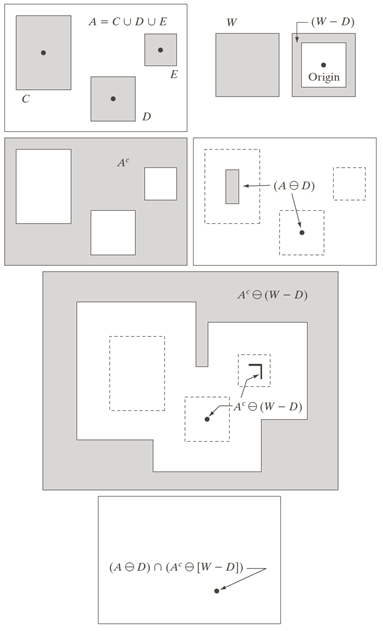
\includegraphics{D:/Documents/GitHub/Commentarii/Digital Image Process Gonzales/1524498629150.png}
\caption{}
\end{figure}

\(\quad\quad\)The approach here is based on an assumed definition that
two or more objects are distinct only if they form disjoint sets, thus
we require each object have at least one-pixel-thick background around
it. If this requirement is not needed, the hit-or-miss transform reduces
to simple erosion.

\subsection{9.5 Some Basic Morphological Algorithms}\label{header-n203}

\(\quad\quad\)One of the principal applications of morphology is in
extracting image components that are useful in the representation and
description of shape.

Boundary Extraction

\[\beta(A)=A-(A\ominus B)\]

where \(B\) is a suitable structuring element.

Hole Filling

\(\quad\quad\)A \emph{hole} may be defined as a background region
surrounded by a connected border of foreground pixels.

Algorithm: \\

\begin{enumerate}
\def\labelenumi{\arabic{enumi}.}
\item
  Initialize \(X_0\) of \(0s\) except at the locations where the given
  point corresponds to a hole.
\item
  \emph{Conditionally dilate}
  \(X_k=(X_{k-1}\oplus B)\cap A^c \quad k=1,2,3,...\), where \(B\) is a
  \(3\times 3\) cross
\item
  Terminate if \(X_k=X_{k-1}\) 
\item
  Compute \(X_k\cup A\)
\end{enumerate}

The intersection at each step with \(A^c\) limits the result to inside
the region of interest.

\end{document}
